%File: formatting-instruction.tex
\documentclass[letterpaper]{article}
\usepackage{aaai}
\usepackage{times}
\usepackage{helvet}
\usepackage{courier}
\usepackage{graphicx}
\frenchspacing
\setlength{\pdfpagewidth}{8.5in}
\setlength{\pdfpageheight}{11in}

%\documentclass{aamas2013}
\usepackage{amsfonts}
\usepackage{amsmath}
\usepackage{algorithmicx}
\usepackage{algpseudocode}
\usepackage{algorithm}

%\fontsize{24}{6}
%\selectfont

\DeclareMathOperator*{\argmin}{argmin}

\pdfinfo{
/Title Using Reward/Utility Based Impact Scores in Partitioning
/Author William Curran, Adrian Agogino, Kagan Tumer}
\setcounter{secnumdepth}{0}  

\begin{document}

%\title{Using Reward/Utility Based Impact Scores in Partitioning}


%\titlenote{For use with aamas2011.cls}}

% AUTHORS


\title{Using Reward/Utility Based Impact Scores in Partitioning}
\author{%William Curran \\
%Oregon State University \\
%Corvallis, Oregon \\
%curranw@onid.orst.edu \\
%\And
%Adrian Agogino \\
%NASA AMES Research Center \\
%Moffet Field, California \\
%adrian.k.agogino@nasa.gov \\
%\And 
%Kagan Tumer \\
%Oregon State University \\
%Corvallis, Oregon \\
%kagan.tumer@oregonstate.edu \\
}

%William Curran\\
%       \affaddr{Oregon State University}\\
%       \affaddr{Corvallis, Oregon}\\
%       \affaddr{curranw@onid.orst.edu}
%\alignauthor
%Adrian Agogino\\
%       \affaddr{NASA AMES Research Center}\\
%       \affaddr{Moffet Field, California}\\
%       \affaddr{adrian.k.agogino@nasa.gov}
%\alignauthor 
%Kagan Tumer\\
%       \affaddr{Oregon State University}\\
%       \affaddr{Corvallis, Oregon}\\
%       \affaddr{kagan.tumer@oregonstate.edu}


\maketitle


\begin{abstract}
Reinforcement learning with reward shaping is a natural approach to solving large multiagent domains with agents who must cooperate to achieve some system objective. However, reward shaping can be computationally expensive to compute. Agent partitioning can assist in this computational complexity by treating each partition of agents as an independent problem. In this paper we introduce a novel agent partitioning approach called Reward/Utility-Based Impact (RUBI). RUBI finds an effective partitioning of agents while requiring no prior knowledge about the domain, leads to better performance by discovering a non-trivial agent partitioning, and leads to faster simulations. We test RUBI in the Air Traffic Flow Management Problem (ATFMP), where there are simultaneously tens of thousands of aircraft affecting the system and no intuitively accurate similarity metric between agents. When partitioning with RUBI in the ATFMP, there is a 37\% increase in performance, with a 510x speed up per simulation step over non-partitioning approaches. Additionally, RUBI matches the performance of the current ATFMP gold standard using no prior knowledge and performing each learning step 10\% faster.

\end{abstract}


%\category{I.2.11}{Distributed Artificial Intelligence}{Intelligent Agents}
%\terms{
%Algorithms, 
%%Management, 
%%Measurement, 
%Documentation, 
%Performance, 
%Design, 
%Economics, 
%Reliability%, 
%Experimentation%, 
%Security, 
%Human Factors, 
%Standardization, 
%Languages, 
%Theory, 
%Legal Aspects, 
%Verification.
%}
%\keywords{Multiagent Partitioning, Multiagent Learning}






\section{Introduction}
Two key elements in a multiagent reinforcement learning system is minimizing computation time and maximizing coordination. Reward shaping is a field in multiagent reinforcement learning that focuses on the design of rewards, and has been shown to assist in multiagent coordination. This reward shaping is typically at a large cost to computation time, and in large, highly coupled domains reward shaping quickly becomes computationally intractable. 

Modeling the reward shaping technique \cite{Proper:2012:MDR:2343896.2344025} in relatively large domains (approx. 400 agents) can be applied to great effect, but requires tens of thousands of randomly generated examples to obtain these approximations. On the other hand, partitioning agents into hierarchies \cite{tumer-holmesparker_ala12} or teams \cite{Curran:2013:AHC:2484920.2485183} speeds up computation time for extremely large domains (approx. 10000-40000 agents) while still using the pure reward shaping technique. While creating these hierarchies or teams, a fundamental understanding of how agents are coupled must be employed by the algorithm designer. In complex domains where the amount of impact an agent has on another is unknown, or in a situation where the algorithm designer has no domain knowledge, these approaches cannot be used. 

In this paper we introduce Reward/Utility Based Impact (RUBI) scores. RUBI learns an effective partitioning of agents, while requiring \textit{no domain knowledge}. It asks the question: What is each agent's local reward with agent $a$ and without agent $a$? The difference in these two rewards is the impact on one agent to agent $a$. This impact is computationally inexpensive to calculate and can be used as an accurate similarity metric that can be used in an off the shelf clustering algorithm. 

We test RUBI in the Air Traffic Flow Management Problem (ATFMP) and use the approach developed by Curran et al. \cite{Curran:2013:AHC:2484920.2485183} and Agogino and Rios \cite{Agogino:2009:EEM:1570256.1570258,Rios}. In this domain the goal is to minimize both congestion and delay associated with the air traffic in the United States. Because the airspace has many connections from one airport to another, the congestion and associated delay can propagate throughout the system. Delays may be imposed to better coordinate aircraft and mitigate the propagation of congestion and the associated delay, but which aircraft should be delayed? The search space in such a problem is huge, as there are tens of thousands of flights every day within the United States \cite{faa05}.

In the ATFMP, multiagent coordination with reward shaping becomes a computationally intractable task, therefore related work has applied automated agent partitioning to reduce the overhead associated with the hard constraint while computing rewards \cite{Agogino:2009:EEM:1570256.1570258,Curran:2013:AHC:2484920.2485183,Rios}. In that work, agents were only required to compute the reward relative to other agents within their partition, removing thousands of extra computations per learning step. We employ this approach, but use RUBI-based partitioning rather than the related work domain-based partitioning.

%A high level view of the approach is as follows: First, we compute partitions of agents. These partitions are treated as reward independent of each other, and therefore need to only compute rewards relative to the other agents within their partition. We will use the term \textit{reward independent} to denote one partition of agents to have no impact on the reward of other partitions. Essentially, no matter what actions one partition of agents take, it will not affect the the action choice for any agent in another partition. We then perform multiagent reinforcement learning using the difference reward. Lastly, we follow the related work approach by adding a greedy scheduler, algorithmically removing all congestion from the system at the cost to delay. Combining the multiagent reinforcement learning with reward shaping and the greedy scheduler turns this into a computationally intractable task. However, with agent partitioning, rewards can be computed many times faster with minimal performance degradation.
 
The contributions of this work are:
\begin{itemize} 
\item Generality: RUBI requires no prior knowledge of the domain, essentially treating the domain as a black box to obtain rewards from.
\item Ease-of-use: RUBI removes the need to derive similarity metrics, removing the need for domain experts in situations where a domain expert isn't available.
\item Performance: RUBI discovers non-trivial agent partitioning through the concept of using a reward function to partition agents.
\item Speed: RUBI leads to a larger number of partitions without losing performance, leading to more independence and therefore faster simulations.
\end{itemize} 
 
The remainder of this paper is organized as follows. Section 2 describes the related work in agent partitioning, the ATFMP, multiagent coordination and reward shaping. In Section 3 we describe the experimental approach taken using multiagent coordination, the difference reward, the greedy scheduler and agent partitioning. Section 4 contains the key contribution of this work, RUBI, and describes the basic algorithm, defines reward-based impact and when to use it, and the key benefits of RUBI. Experimental results are then provided in Section 5, followed by the conclusion and future work in Section 6.

\section{Background}
\label{sec:BACKGROUND}

To motivate our approach, we introduce previous work performed in the field of agent partitioning, a description and overview of the ATFMP, and describe the reward shaping technique used in this work.

\subsection{Agent Partitioning}

Previous work in agent partitioning has focused on what specifically to partition. Jordan and Jacobs \cite{716791} developed the Hierarchical Mixtures of Experts (HME) method to partition the state space directly, such that different agents can focus on specific regions of the state space. This method works well in non-linear supervised learning tasks. In this work all learning is unsupervised, so this technique cannot be used.

Partitioning actions so that each agent is responsible for a small number of actions is another approach used often. Sun and Pearson \cite{Sun98someexperiments} divided actions into two types, speed and turn, and each type was handled by a separate agent. This approach uses domain knowledge, and partitioning actions applies well in robotics, but not in domains where all actions need to be explored.

The last partitioning technique we describe is to partitioning system-level goals into smaller tasks. In the work by Dayan and Hinton \cite{Dayan93feudalreinforcement}, they accomplished goal partitioning through task allocation, where agents are organized in a hierarchy, where high-level agents assign goals to agents lower in the hierarchy on-line. In the work by Reddy and Tadepalli \cite{Reddy_learninggoal-decomposition}, the approach is more structured. In this work the partitioning of the goal is learned through externally provided examples. Overall, these approaches are under the assumption that the system-level goal can be subdivided, which is not always the case. 

In this work, we partition agents, essentially treating each partition of agents as an independent problem. Agents from one partition could potentially affect the environment of agents in another partition, but this work attempts to minimize the partition overlap. In a partitioning with complete reward independence, this work essentially treats the problem as a set of smaller and easier independent problems.


\subsection{Air Traffic Flow Management Problem}

The ATFMP addresses the congestion in the National Airspace (NAS) by controlling ground delay, en route speed or changing separation between aircraft. The NAS is divided into many sectors, each with a restriction on the number of aircraft that may fly through it at a given time. This number is formulated by the FAA and is calculated from the number of air traffic controllers in the sector, the weather, and the geographic location. These sector capacities are known as en route capacities. Additionally, each airport in the NAS has an arrival and departure capacity that cannot be exceeded. Eliminating the congestion in the system while keeping the amount of delay each aircraft incurs small is the fundamental goal of ATFMP. 

%Two popular approaches to simulating the ATFMP had been to develop Lagrangian models of each aircraft's dynamics, and to create aggregate models of the NAS \cite{Bertsimas:1998:ATF:767667.768027, Bilimoria, McNally, Mueller_analysisof}. In the Lagrangian model approaches, typically the trajectories of each aircraft are taken into account and either collision-avoidance or congestion-reduction is performed \cite{Bilimoria, McNally}. This is an accurate and fine-grained approach to the ATFMP, but also time-intensive and complex. On the other hand, aggregate models have been shown to simplify the NAS and therefore are a much simpler approach to the ATFMP. The aggregate models have been used in conjunction with linear programming to find solutions to air traffic flow \cite{Bertsimas:1998:ATF:767667.768027}, and linear algorithms to analyze departure, enroute and arrival delays \cite{Mueller_analysisof}.

In this work we chose to use an aggregate model of the NAS. By choosing to control the ground delay of each aircraft, rather than the enroute speed, and using historical NAS flight data, we only need to count how many aircraft are within a particular sector at a particular time. Actions affect the simulation minimally, as an aircraft with imposed ground delay simply needs to shift its entire flight plan by the amount of ground delay, greatly speeding up simulation time.

%Previous work in the ATFMP and scheduling had applied Integer Linear Programming \cite{Bertsimas}, evolutionary approaches \cite{Agogino:2009:EEM:1570256.1570258, Rios}, and multiagent approaches \cite{tumer-agogino_jaamas12,Curran:2013:AHC:2484920.2485183, 664154, Sislak:2008:AMA:1402744.1402755, Zhang95areinforcement}. The ATFMP is a naturally distributed problem with complex interactions among all aircraft and airports. This renders predetermined centralized solutions suboptimal whenever there is any deviation from the expected air traffic flow. Therefore using a decentralized multiagent system is an ideal approach in such a domain.

%There are three main issues to using Integer Linear Programming (ILP) that are removed using a multiagent approach; first, designing an ILP algorithm for a particular task is a difficult process, and it takes a lot of effort to adapt ILP to new problem variations that inevitably come up. Second, a formulation of ILP is complex even for simple problems. For real world implementations there is an enormous amount of subtle complexity that has to be included in the system, such as balancing the needs to airlines, air traffic controllers and passengers. These complexities can be added in a straightforward way in reward functions, but not in ILP. Third is computational complexity; ILP computation can grow exponentially with problem size. A carefully designed ILP can avoid this exponential increase within a certain range of parameters, but after a certain problem size, computing an ILP solution is infeasible, making it impracticable for the full ATFMP.

The approach we use in the ATFMP follows the same approach by Curran et al. \cite{Curran:2013:AHC:2484920.2485183} and Agogino and Rios \cite{Agogino:2009:EEM:1570256.1570258,Rios}. Rather than treating congestion as a soft constraint, these approaches removed congestion completely from the system algorithmically through the use of a greedy scheduler. A high level view of this approach is as follows: First, they computed partitions of agents using a domain-based similarity metric of sector overlap and hierarchical agglomerative clustering. These partitions are treated as reward independent of each other, and therefore need to only compute rewards relative to the other agents within their partition. We will use the term \textit{reward independent} to denote one partition of agents to have no impact on the reward of other partitions. Essentially, no matter what actions one partition of agents take, it will not affect the the action choice for any agent in another partition. They then performed multiagent reinforcement learning using the difference reward. Lastly, they introduced a greedy scheduler, removing all congestion from the system. They found that combining the multiagent reinforcement learning with reward shaping and the greedy scheduler turns this into a computationally intractable task. They solved this problem with agent partitioning, showing that rewards can be computed many times faster with minimal performance degradation.

%\subsection{Heterogeneous bar problem}
%We introduce a modification to the bar problem where agents can go only a subset of nights.

%\subsection{Hierarchical reinforcement learning}
%Agent hierarchies are essentially what we are doing. We use hierarchical reinforcement learning to solve this problem. We decompose %the problem into a bunch of smaller problems. This is like Dietterich et. al.



\subsection{Reward Shaping}
Multiagent coordination is an important aspect of many domains, such as data routing \cite{tumer-wolpert_jair02}, air traffic control \cite{tumer-agogino_jaamas12}, Robocup soccer \cite{AAMAS12-agmon}, rover coordination \cite{5509316} and power plant operations \cite{Colby:2012:SFF:2343576.2343637}. A learning or evolutionary algorithm will often convert a once computationally intractable search problem into a feasible guided search. 

In learning algorithms, reward design is important in keeping convergence time low while keeping performance high. In many multiagent coordination domains there is a difference between maximizing the system-level reward and maximizing a single agent's reward. If an agent always takes the locally-optimal action, it does not always maximize the system-level reward; a common example of this is the Tragedy of the Commons \cite{Hardin}.

The difference reward \cite{tumer-wolpert_jair02} is evaluated such that each agent's reward is related to the individual's contribution to team performance, therefore the signal-to-noise ratio is improved considerably. This leads to final better policies at an accelerated convergence rate, as well as overcoming the Tragedy of the Commons. The difference reward is defined as:
%
\begin{equation}
D_i(z) = G(z) - G(z - z_i + c_i)\;,
\end{equation}
%
where \textit{z} is the system state, $z_i$ is the system state with agent $i$, and $c_i$ is a counterfactual replacing agent $i$. This counterfactual offsets the artificial impact of removing an agent from the system. For example, removing an aircraft from the system always artificially decreases the amount of congestion and delay, which would provide a poor reward if a counterfactual is not used.

The difference reward provides a compact encapsulation of the agent's impact on the system. It reduces the noise from other agents in the reward signal and has outperformed both system-level and local rewards in many congestion domains \cite{AAMAS12-agmon,Agogino:2012:ELS:2330163.2330306,Colby:2012:SFF:2343576.2343637,tumer-wolpert_jair02}. In many systems it is difficult or impossible to calculate the difference reward without resimulation, which can become prohibitively costly. If resimulation is fast, or the difference reward function is easily approximated, this reward function is a powerful tool for multiagent coordination.

\section{ATFMP Approach}

In this section we give a brief overview of the learning approach used in this paper. This application approach is not a key focus of this work and was developed by Curran et al. \cite{Curran:2013:AHC:2484920.2485183} and Agogino and Rios \cite{Agogino:2009:EEM:1570256.1570258,Rios}, and the reader is referred to this related work if they have any additional questions.

\subsection{Agent Definition}
In this paper, agents are assigned to one of 35,844 aircraft with cooperation enforced by airport terminals. Cooperation needs to be enforced because aircraft are naturally greedy. Aircraft are owned by different companies, and those companies are not interested in making sure aircraft from other companies arrive on time. This enforced cooperation assumption by aircraft terminals (or the government) is essential to remove greedy aircraft from the system.

Aircraft flight plans are from historical flight data from the FAA. Therefore, the only aspect of the environment we can change is the ground delay for each aircraft. Agents may select a certain amount of ground delay from 0 to 10 minutes (11 actions) in the beginning of every simulation. The FAA data has the sector location of each plane for every minute that plane was in service. Therefore, adding ground delay simply shifts a plane's flight plan over by that many minutes. The greedy scheduler then takes all plane flight plans, checks if the flight plans cause any congestion, and then further delays planes to eliminate congestion from the system.

In this formulation, agents do not have the capability to change their action based upon the system once the simulation starts, therefore feedback can only be given once per simulation. Since agents are given no knowledge of the environment, they have no state. This simplifies the learning problem for each agent, as they only have eleven actions to sample from, but complicates the coordination. Agents must choose an action without prior knowledge of other agents choices, and must learn how the environment is changing, and simultaneously what action to take.

Agents learned using Action-Value Learning with a zero initialized value table. This is a stateless approach where agents map actions to values representing the quality of that action. 

%\subsection{Agent Learning}


%In single-agent systems, agents employing the exploration-exploitation strategies eventually come to an optimal solution \cite{Sutton98reinforcementlearning}. In multiagent systems the exploration of other agents become an issue. When an agent takes a greedy action, other agents can learn how that affected the environment, and modify their own greedy action. When an agent takes an exploratory action rather than a greedy action, other agents modify their greedy action based on how the environment changed with the exploratory actions. Agents learn to compensate for the exploratory actions in the system, so when exploration removed after some learning performance often decreases. This behavior is caused by exploratory noise \cite{holmes-aamas}.

%With so many agents in this system, exploratory noise causes a large problem. In the beginning of learning, having a large exploration is beneficial for the system. With 10\% of the agents taking random actions, we can find a good area of the reward space to explore. But near the end of learning, with most agents almost converged to a nearly optimal solution, 10\% of agents are taking random actions, causing over 3,500 agents to introduce noise into the learning of all other agents. To circumvent this problem, we need to have more agents performing greedy action selection as during each consecutive learning step. Therefore, $\epsilon$ would need to be lowered throughout learning to accomplish this. We approached this problem by reducing $\epsilon$ every n time steps by a constant amount (more sophisticated techniques such as the Boltzmann equation could be used, but only simple $\epsilon$ reduction was needed). The following equation was applied to $\epsilon$ at every time step:

%\begin{equation}
%\epsilon = \epsilon * c^{t * \Theta(t \mod n)}\;,
%\end{equation}
 
%where c is a constant value (typically .99), $t$ is the current time step and $\Theta(t \mod n)$ is a step function that equals 1 when $t \mod n$ is 0 and 0 otherwise, and $n$ is a value that varied depending on the number of learning steps. With more learning steps $n$ was higher, and in experiments with fewer learning steps $n$ was lower.

\subsection{Reward Structures}

In this section we first develop the system-level reward. This reward represents how well the system as a whole is performing. We want this value to be as high as possible. We then develop the difference reward from the system-level reward. The difference reward represents how much a particular agent contributes to the system-level reward. Agents should be rewarded with the difference reward, and system performance should be measured as the system-level reward. 

The system-level reward in the ATFMP developed focuses on the cumulative delay ($\delta$) and congestion ($C$) throughout the system:
%
\begin{equation} \label{eq:Global}
G(z) = -(C(z) + \delta(z))\;,
\end{equation}
%
where $C(z)$ is the total congestion penalty, and $\delta(z)$ is the cumulative system delay.

The total congestion penalty is the sum of differences between sector capacity and the current sector congestion. The total delay is the sum of delays over all aircraft. This is a linear combination of the amount of ground delay and the amount of scheduler delay an agent incurred.

Agogino and Rios originally had the idea of adding a greedy scheduler to algorithmically remove congestion from the system, while simultaneously using learning to minimize delay. We follow this approach, and therefore our system-level reward is simply:
%
\begin{equation} \label{eq:Global}
G(z) = -\delta(z)\;
\end{equation}
%
With so many agents, tens of thousands of actions simultaneously impact the system, causing the reward for a specific agent to become noisy with the actions of other agents. An agent would have difficulty learning an optimal solution using such a noisy reward signal. A difference reward function reduces much of this noise, and is easily derived from the system-level reward:
%
\begin{equation}
D_i(z) = \delta(z-z_i + c_i) - \delta(z)\;,
\end{equation}
%
where \textit{$\delta(z-z_i + c_i)$} is the cumulative delay of all agents with agent $i$ replaced with counterfactual \textit{$c_i$}.

We used a non-zero counterfactual for two reasons. One, when an aircraft is removed from the system, the reward given to the agents is artificially increased. Furthermore, the aircraft are less likely to cause conflicts due to the easier scheduling problem. Two, we used a counterfactual where the agent does not delay at all, meaning that if not delaying produces a higher reward than delaying, this should be found quickly. We also take advantage of the fact that most airplanes do not need to be delayed. If the counterfactual is equal to the agent removed, the difference reward becomes zero and does not need to be calculated, thus speeding up reward calculations.

\section{RUBI}
In this section we will describe in detail the Reward/Utility-Based Impact (RUBI) algorithm. We will first describe a general overview of RUBI, and the implementation. We will then go over the variety of ways RUBI impact scores and simulations can be developed. Lastly we will give an overview of the benefits of using RUBI.

\subsection{RUBI Basics}
In this work we introduce an autonomous partitioning algorithm requiring no domain knowledge, the Reward/Utility Based Impact algorithm. Domain-based partitioning directly looks at aircraft flight plans and partitions agents together based on how similar their flight plans are. Instead, we develop an initial agent similarity matrix that uses no knowledge about the domain, and partitions agents together based on the impact of one agent to another. This matrix can then be used as an input to a hierarchical agglomerative clustering algorithm. Additionally, by removing all knowledge about the domain and partitioning based on reward, RUBI can be used to discover non-trivial indirect interactions encoded in a reward signal.

On a basic level, this algorithm leverages the same central idea behind difference rewards: If an agent is removed from the system, how does that affect system-level reward? We modify this approach to answer the question: If an agent is removed from the system, how does that impact other agents? If one agent's action heavily impacts another agent's reward (positively or negatively), those agents are coupled enough to be partitioned together. The RUBI algorithm computes a localized reward for each agent with agent $i$ in the system, and then compares that reward to the localized reward for each agent if agent $i$ is not in the system. This partitioning algorithm is based around the central idea:

\begin{align}
|L_i(z) - L_i(z-z_j)| &> |L_k(z) - L_k(z-z_j)|   \Rightarrow \\
SIM(i,j) &> SIM(k,j) \nonumber
\end{align}

where $L_i(z-z_j)$ is the localized reward of agent $i$ if $j$ is not in the system, $L_k(z-z_j)$ is the localized reward of agent $k$ if $j$ is not in the system, and $L_i$ and $L_k$ are the localized rewards of $i$ and $k$ when all agents are in the system. This means that if the localized reward of agent $i$ changes more than the localized reward of agent $k$ when agent $j$ is taken out of the system, agent $j$ has more effect on agent $i$ than agent $k$. This is the essential idea behind RUBI, and is encoded in this algorithm through the equation:
%
\begin{equation} \label{eq:RUBI Update}
C_{r,a} \leftarrow C_{r,a} + |L_a(z) - L_a(z-z_r) | \;,
\end{equation}
%
where $L_a(z)$ is the reward agent $a$ receives when all agents are in the system, $L_a(z-z_r)$ is the reward agent $a$ receives with agent $r$ not in the system, and $C_{r,a}$ is the cumulative impact agent $r$ has on agent $a$.

\subsection{Implementation of RUBI}
The RUBI algorithm (Algorithm 1) first initializes an $N$ x $N$ matrix $C$, where $N$ is the number of agents within the system. It then calculates actions based on the $ACT()$ function, which is typically random action selection. A simulation is then ran with all of the agents in the system and the localized reward is calculated for every agent. We then remove an agent from the system, recalculate the reward for each agent (since this is a localized reward, this is typically a fast operation), and update the impact table based on equation \ref{eq:RUBI Update}. This is a high level understanding of RUBI, and the following sections will explain how the impact data is computed, simulation specifics, the $ACT()$ function, and finally when this partitioning algorithm is practical.

\begin{algorithm} \label{alg:RUBI}
  \caption{Reward/Utility Based Impact Algorithm}
  \begin{algorithmic}[1]
    \Statex
    \Function{RUBI}{$sim$}
      \State{$C \leftarrow N x N$}
	  \For{$i \leftarrow 1$ to $iterations$}     
	    \State{$actions \leftarrow ACT()$}
	    \State{$sim.run(actions)$}
	    \State{$L(z) \leftarrow sim.getRewards()$}      
		\For{$r \leftarrow 1$ to $N$}
			\State{$sim.removeAgent(r)$}
			\State{$L(z-z_r) \leftarrow sim.getRewards()$}
			\For{$a \leftarrow 1$ to $N$}
				\State{$C_{r,a} \leftarrow C_{r,a} + |L_a(z) - L_a(z-z_r) |$}
				\EndFor
			\State{$sim.addAgent(r)$}
		\EndFor
	\EndFor        
    \EndFunction
  \end{algorithmic}
\end{algorithm}

\subsection{Reward/Utility based impact}
The impact data used to compute the similarity matrix is obtained from a localized reward or utility with respect to an agent. Learning in congestion problems using local rewards typically lead to a terrible solution, as local rewards correspond to greedy agents. Congestion problems usually need a few agents to receive negative rewards in order for the rest of the agents to receive positive rewards. Greedy agents do not take this into account. In RUBI, we do not want to learn, but instead analyze the local impact one agent has on another, therefore local rewards are an ideal choice.

In this work we apply RUBI only to reinforcement learning, therefore all impact scores are based on reward, but the work applies to algorithms that use utilities. A traditional local reward can work, or a localized reward can be specifically built for the partitioning. A high-level reward, such as the system-level reward, will not work as impact data. When computing the difference in the global reward with all agents and the global reward without a specific agent, we compute the difference reward. The difference reward represents how much an agent impacts the system, but the goal here is to find how much one agent impacts another agent.

Equation \ref{eq:RUBI Update} is simply an accumulation of impact scores. Given enough iterations, this accumulation is informative enough to perform accurate partitioning. In this research we are interested more in the relative impact score from one agent to another, rather than what the explicit impact score is. This iterative approach requires at minimum enough iterations to evenly distribute over all actions an agent can take. Ideally each action should be sampled many times for a accurate impact estimate. Future work in RUBI involves approximating the impact score of each agent by adding a learning rate and subtracting off previous impact scores per iteration. This causes $C_{r,a}$ to converge to an impact score, and analyzing this impact score may be useful in team formation or domain analysis.

%When we performed partitioning in the heterogeneous bar problem we use a local reward that was simply the local version of the system-level performance:

%\begin{equation}
%R = e^{-x_i(z)/c} \;,
%\end{equation}

%where $x_i(z)$ is the attendance on the night that agent $i$ went to the bar. Looking at Equation \ref{eq:BarProblem-Local} you can %see that this a local reward for the heterogeneous bar problem, and an example of using a local reward for partitioning data.

For the ATFMP we developed a partitioning reward by both simplifying the simulation and adding to the reward. At a high level we want to encapsulate how one agent affects another in the reward. We took out the greedy scheduler and used the congestion as added information for the similarity data:
%
\begin{equation} \label{eq:RUBI ATFMP-L}
R = -(C(z) + \delta(z))\;,
\end{equation}
%
where \textit{C(z)} is the congestion penalty and \textit{$\delta$(z)} is the delay as defined in section 3.2. This is a perfect example of how different the simulation can be during partitioning than during learning.

\subsection{Simulation}
The simulation is also an aspect that can be widely varied when using RUBI. One example already explored is the ATFMP reward-based impact data, where we change the simulation by removing the greedy scheduler, and taking advantage of the congestion information. This concept can be expanded upon by borrowing some of the concepts from transfer learning.

Transfer learning is a traditional approach used in both classification and learning to apply what is classified or learned from a smaller and easier domain to a larger more complicated domain. One subset of transfer learning is transfer clustering. Given a proper mapping, clusters learned in a small simulation can be applied to a larger simulation \cite{6378284}. We can apply the same concepts developed in transfer clustering to this RUBI simulation. We've shown the simulation used during partitioning doesn't necessarily have to be the same as the simulation used during learning. It's also intuitive that any simulation can be used during partitioning, as long as there is a mapping from the RUBI simulation to the learning simulation. This approach is very beneficial in domains where the simulation is costly and a mapping can be discovered. 

The $ACT()$ function returns a list of agent actions to use in the RUBI simulation. This is yet another aspect of this algorithm that can be chosen by the user. In the domains with no failure modes, this function typically returned random actions. The fundamental goal of $ACT()$ is to have as much of the interactive state space explored as possible, but we cannot exhaustively search the entire state space, as that would be both impractical and computationally impossible. For this reason we choose to take random actions. When random actions are taken, agents are not driven by any motivating logic, and impact scores will be biased only toward agents who consistently impact each other. 

There are many domains, such as robotics, where random actions may cause certain failure modes, or where agents need to be in a particular area of the state space before interactions can really be analyzed. In these domains the $ACT()$ function can either sub-sample from a set of known non-failure mode actions, or be replaced with an actual learning algorithm to get the agent in a successful area of the state space before sampling. 

\vspace{14mm}
\subsection{Benefits of RUBI}
One of the key strengths of RUBI is its sheer simplicity and generality combined with computing highly informative similarity scores, leading to well-performing partitions, as described in the results section. It needs no prior knowledge about the domain to perform partitioning, and simply needs a localized reward from each agent to build the similarity matrix. This makes RUBI highly generic and can be applied to any multiagent domain. It can treat the multiagent system as a black box, giving it random actions and receiving rewards. It can also discover non-trivial agent coupling. 

Since RUBI uses a localized reward as partitioning data, any effect one agent has on another agent will be encoded in this reward. For example, if an agent $a$ is removed from the system, and agent $b$'s reward changes, it means that in some way agent $a$ affects agent $b$ in a direct or indirect way. This indirect affect can be captured by RUBI and used as additional information when partitioning, leading to higher quality partitions in domains with complex interactions.

One of the key benefits of RUBI is that partitions built using RUBI are likely to be greater in number without loss of performance. The ATFMP is a perfect example. Domain-based partitioning based on similar sectors encodes how often two aircraft can impact each other. RUBI on the other hand looks more into how the actions of one agent impact another agents reward, in this case congestion. For example, plane $a$ and plane $b$ go through the same sectors, but are never congested. Using domain-based partitioning, two agents that go through the same sector many times would be partitioned together, so plane $a$ and plane $b$ would be partitioned together. In partitioning using RUBI, if over a few thousand trials the congestion of each plane is always 0, those planes actions never impact each others rewards, therefore they would not be partitioned together. The same is true if the congestion of each plane remains the same non-zero value, the actions do not affect the reward, therefore they are not partitioned. This is a very important key feature of RUBI, and leads partitioning using RUBI to find more partitions without loss of performance. It is a perfect example of RUBI finding a non-trivial partitioning.


\section{Results}

During preliminary analysis, RUBI works as expected in simple toy problems, but what happens when we apply it in a complex domain with tens of thousands of agents, such as the ATFMP? When RUBI is applied during partitioning in the ATFMP, simulation time decreases and the ease of application raises over developing a similarity metric. The removal of domain knowledge allows the same RUBI algorithm to be used in simple problems as well as the ATFMP with no effort and without any need to develop a similarity metric. The approach used here is the same as in Curran et al. \cite{Curran:2013:AHC:2484920.2485183} and Agogino and Rios \cite{Agogino:2009:EEM:1570256.1570258,Rios}, except utilizing RUBI.

Partitions developed using RUBI uses similarity metrics that encapsulated the agent coupling. In this section we will first show how RUBI partitioning works well in the ATFMP, and analyze the cost/benefit of varying the number of partitions. We will then compare RUBI-based partitioning to domain-based partitioning and see that RUBI develops better quality partitions as well as partitions that lead to faster simulation times.


\subsection{RUBI Performance in the ATFMP}

\begin{figure}
\centering
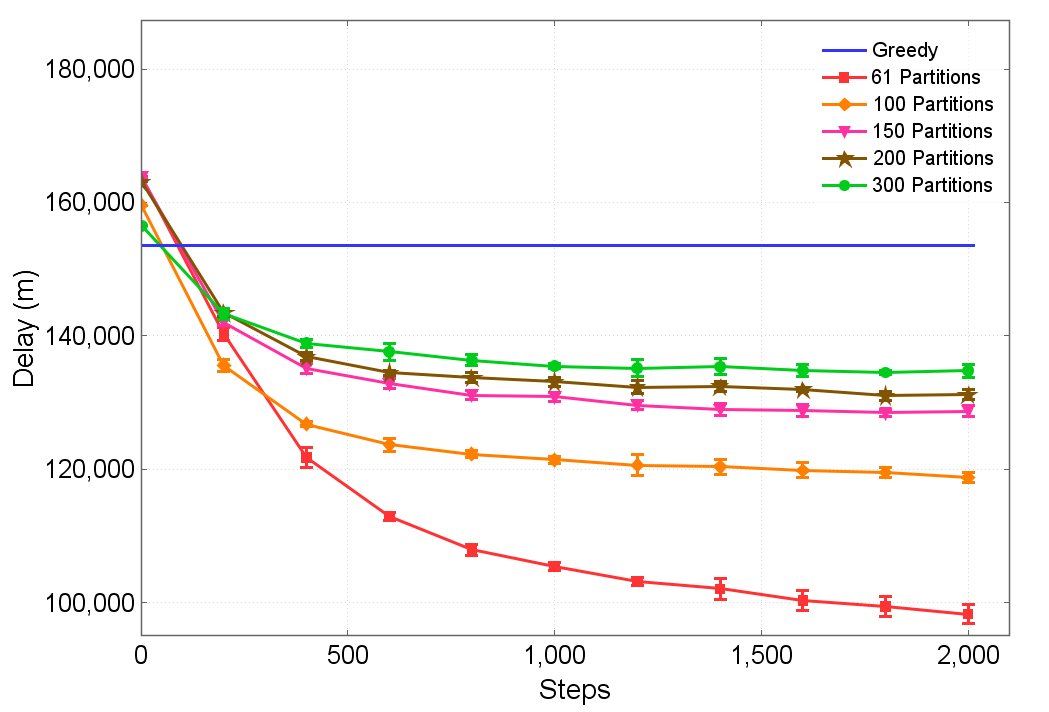
\includegraphics[width=1.0\columnwidth]{ATFMPNewvsGreedy}
\caption{As the number of partitions decreases, performance improves while time complexity increases. Note that a reward independent partitioning using RUBI includes 61 partitions. }
\label{ATFMPNewvsGreedy}
\end{figure}


When partitioning agents using RUBI in the ATFMP agents took random actions, the greedy scheduler was not used, and the localized reward for each agent involved both congestion and delay (Equation \ref{eq:RUBI ATFMP-L}). The reward-based impact function included both delay and congestion, since the greedy scheduler was removed, so the difference in delay was constantly 0 when computing reward-based impact. Therefore, agents were partitioned together based on whether their actions cause congestion to other agents. 

Partitioning with RUBI and the difference reward outperformed the greedy scheduler. Figure \ref{ATFMPNewvsGreedy} shows a variety of partitions out performing the greedy scheduler. The final performance of the ATFMP using RUBI-based partitioning was similar to domain-based partitioning performance. This is because at a converged partitioning, all agents are considered reward independent. The key benefit of RUBI-based partitioning was that a reward independent partition involved 61 partitions, but in domain-based partitioning the smallest was 3. This leads to faster processing time, at no cost to performance. This is discussed in further detail in the next section.

To understand how much overlap partitions had with each other, we analyzed the similarity each partition had with itself, and the average similarity each partition had with other partitions. Similarity was defined as the similarity metric used in domain-based partitioning, the number of similar sectors between agents.

In this section, we find the number of sectors that are similar between planes in a partition (self-similarity). We then find the the average number of sectors each plane in one partition has in common with each plane in another partition, and average all of these together to obtain a other-similarity metric. When graphing these metrics we take the percentage of self-similarity to other-similarity, and vice-versa. In a purely reward independent partition, the other-similarity is 0, and the self-similarity is 1. As the amount of self similarity increases though, the computation time increases exponentially, and the benefits of partitioning decreases.

The key difficulty in performing partition in the ATFMP, where almost every agent is coupled, is to partition agents in such a way that the similarities between partitions are as small as possible, while still preserving the computational benefits of partitioning. For this reason, we need to analyze both the performance of a variety of partition sizes, as well as the cost associated with the partition sizes.

When partitioning in a multiagent system, unless partitions are reward independent, there is always a cost and a benefit. The benefit is faster simulation time and/or reward calculations at the cost to performance. Although there is always a cost to performance, there is typically a point where the benefit of faster computation offsets the cost to performance. When partitioning with RUBI, with the slowest simulation there is a 37\% increase in performance over the greedy scheduler, with a 510x speed up \textit{per learning step} over non-partitioning approaches, and with a larger number of partitions we obtained 5400x speed up \textit{per learning step} with a 20\% increase in performance.

In the ATFMP, this partitioning benefit speeds up computation by magnitudes, but how much performance are we losing, and at what point is the partitioning costing too much performance for the benefit of faster computation? Figure \ref{NewPartitionComparisons} compares average computation time, final performance and self-similarity of each partition. The average computation time per learning step for each partition size remains static, and then exponentially increases once the self-similarity becomes large. This is the cost of each partition. There is also has a sharp increase in final performance as the self-similarity increases. This is the benefit of each partition. Both of these performance metrics are correlated greatly with the self-similarity metric.

%Graph \ref{ATFMPCostBenNew} shows the benefit/cost ratio for each partition. At 100 partitions the benefit begins greatly outweighing the cost. If performance is important, 50 partitions reaches 80\% of the max performance, at only a 20\% speed up, but if a faster result is more important, 70\% of max performance can be reached with 90\% faster learning steps.

\begin{figure}
\centering
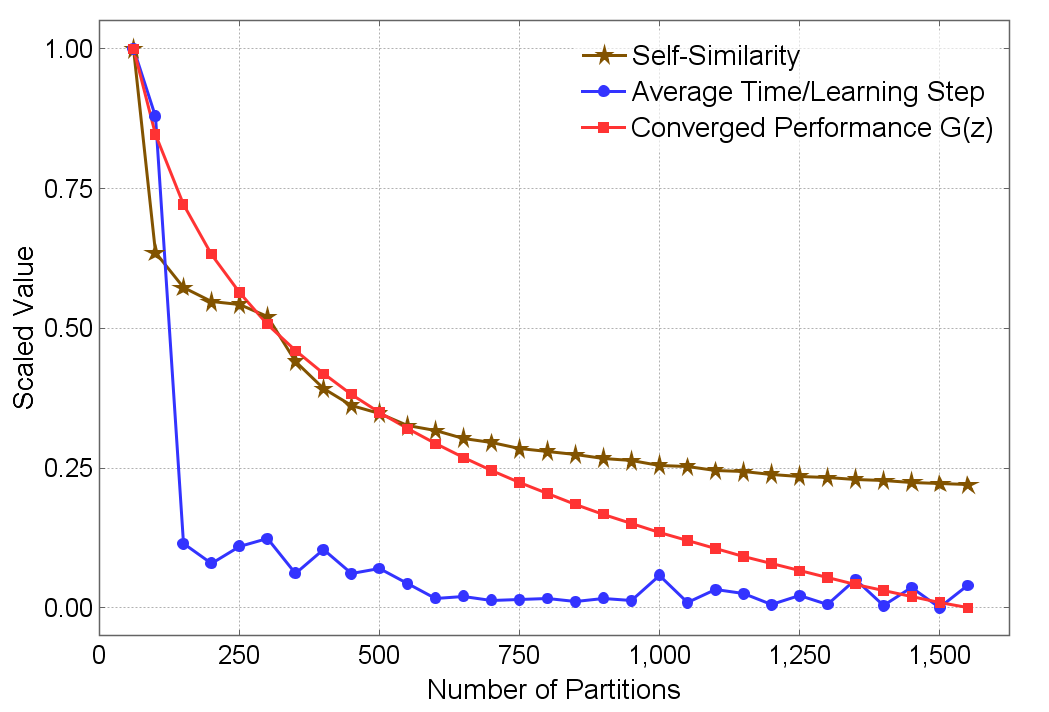
\includegraphics[width=1.0\columnwidth]{NewPartitionComparisons}
\caption{As the self-similarity increases, final performance and time taken per learning step increases. Note that final performance is a 6th degree polynomial trend line with $R^2 = .95$, and all values are scaled between 0 and 1 for comparison purposes.}
\label{NewPartitionComparisons}
\end{figure}

%\begin{figure}
%\centering
%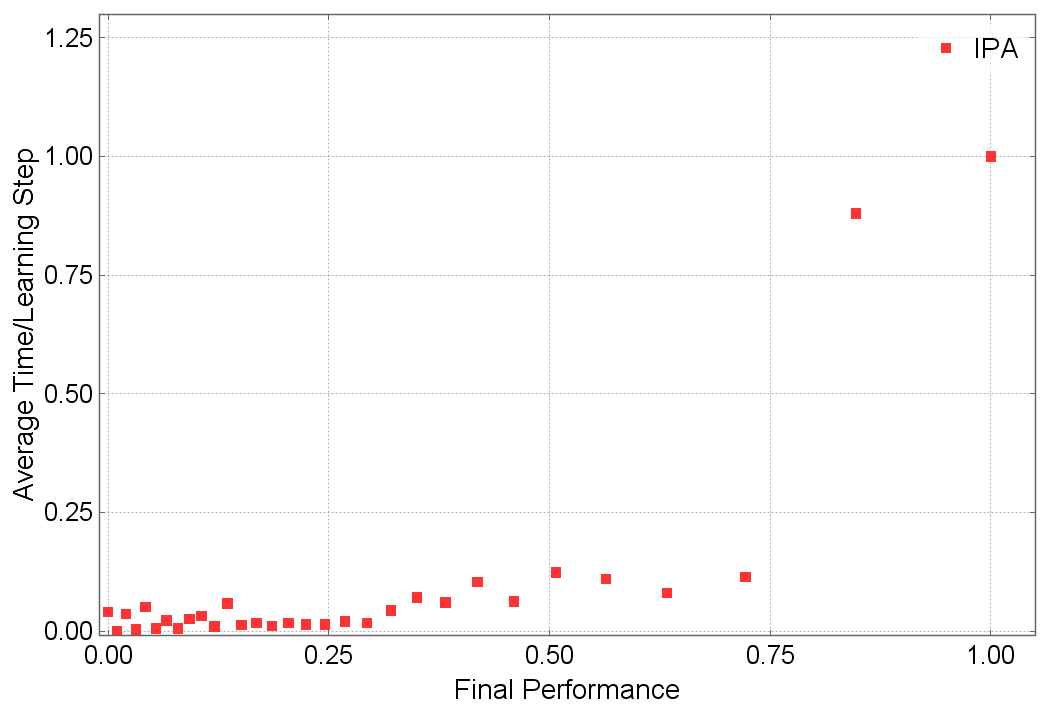
\includegraphics[width=1.0\columnwidth]{ATFMPCostBenNew}
%\caption{}
%\label{ATFMPCostBenNew}
%\end{figure}



\subsection{Comparison Between RUBI and Domain-Based Partitioning}

The comparisons made in this section are made with respect to the similarity metric chosen by Curran et al. \cite{Curran:2013:AHC:2484920.2485183} and Agogino and Rios \cite{Agogino:2009:EEM:1570256.1570258,Rios}, the number of overlapping sectors. One needs to keep in mind that if a group of domain experts in air traffic control worked together to develop a similarity metric, partitioning using that metric is likely to be extremely accurate. RUBI-based partitioning benefits from ease-of-use and generality. With RUBI a very well performing partitioning can be computed with little or no effort.

Partitioning with RUBI developed better similarity scores than domain-based partitioning (Figure \ref{Self-SimOldvsSelf-SimNew}). By partitioning using congestion, the similarity metric was able to represent both similar sectors as well as sector congestion. Consider the case where two aircraft have the same flight plan, excluding their congested arrival and departure location. These aircraft would be partitioned together when using only similar sector domain knowledge. With RUBI, those aircraft would be partitioned together with aircraft that cause them congestion. By partitioning using the impact one agent had on another agents reward, we are able to formulate higher quality partitions, without the overhead of developing similarity metrics or learning domain knowledge.

\begin{figure}
\centering
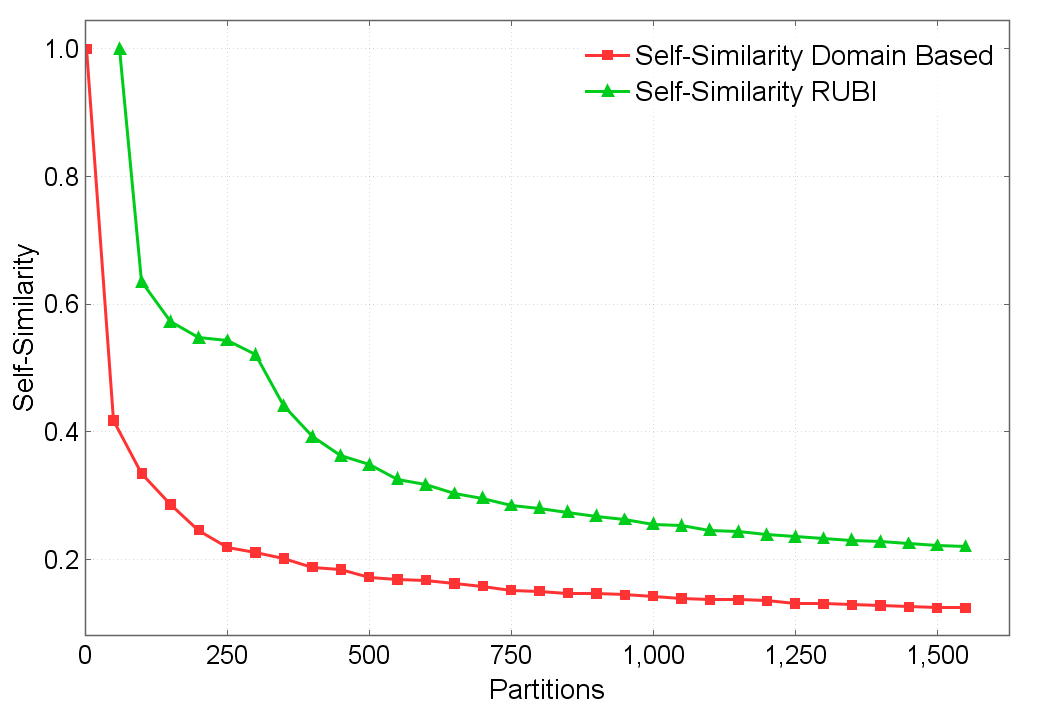
\includegraphics[width=1.0\columnwidth]{Self-SimOldvsSelf-SimNew}
\caption{Partitions formed with RUBI had higher self-similarity than using domain-based partitioning. This leads to higher quality learning with respect to each partition.}
\label{Self-SimOldvsSelf-SimNew}
\end{figure}

In addition to higher self-similarity, the partitioning using RUBI converged to a reward independent partitioning that included many more partitions than domain-based partitioning. In a reward independent partitioning, more partitions reduce the computation while incurring no loss of performance. The reward independent domain-based partition included 3 partitions, while partitioning with RUBI included 61 partitions. This is due to using reward-based impact as a similarity metric, as mentioned in Section 4.3. Two agent's actions may greatly affect each other during simulation, but their reward-based impact on each other might still be zero. This is a very important fact to keep in mind during partition analysis. For example, if two agents go through the same sectors, but neither agent causes another agent more or less congestion, then the difference in local reward will be zero, even though those aircraft affect each other. This leads to more partitions, and faster simulations. This is an example of RUBI finding a non-trivial partitioning.

When comparing final performance, a direct comparison of performance is not adequate. This is because partitions are not evenly distributed, which causes extremely large bias when comparing final performance to number of partitions. To show this in detail, we directly compared performance. We saw that with a larger number of partitions domain-based partitioning initially out performs RUBI, but RUBI began out performing domain-based partitioning with a smaller number of partitions. 

In looking deeper into the reasoning behind this, we realize that partitions are not evenly distributed. Initially, domain-based partitioning have very large partitions compared to RUBI partitioning. This is due to the accumulation of similar sectors in domain-based partitioning. In domain-based partitioning, all of the planes with high overlap are initially merged together, giving domain-based partitioning initially larger partitions. Since this is a highly-coupled domain, this also leads to one partition becoming much larger than others. This is not seen in the self-similarity due to self-similarity being an average of all self-similarities. Basically, domain-based partitioning in this domain results in one partition having very high self-similarity, while other partitions get ignored. Although performance is initially better in domain-based partitioning, it is at 800+ partitions, meaning that the performance at this level of partitioning is already low for both partitioning approaches, and is therefore less useful.

RUBI, which partitions based on the reward of congestion and delay, initially merged together partitions whose reward highly impacted each other, which creates more evenly distributed partitions, leading to a better overall similarity, but initially worse performance. With a smaller number of partitions, RUBI-based partitions end up becoming larger on average. This in turn led to a bias for RUBI partitioning. Note that when all partitions are reward independent, RUBI partitioning included a much smaller average size, and many more partitions.

This results in us comparing final performance to the average size of the top 5\% of partitions. This gives a comparison of how well a partitioning performs with respect to the size of it's partitions, rather than the number. Figure \ref{ATFMPPerformancevsAvgSize} shows that initially in domain-based partitioning, learning performance does not increase with respect to the average size of the partitions. RUBI on the other hand creates a partitioning with constantly increasing performance. One key point of this figure is that RUBI-based partitioning developed a better partitioning with every additional partition merge. This is because RUBI uses rewards to develop an impact score, so when two partitions are merged together it is guaranteed that performance will increase. Domain-based partitioning on the other hand had a steady performance until a certain point, and then performance increased dramatically. Note how many points are sampled for domain-based partitioning in Figure \ref{ATFMPPerformancevsAvgSize} for the smaller sized partitions.

%\begin{figure}
%\centering
%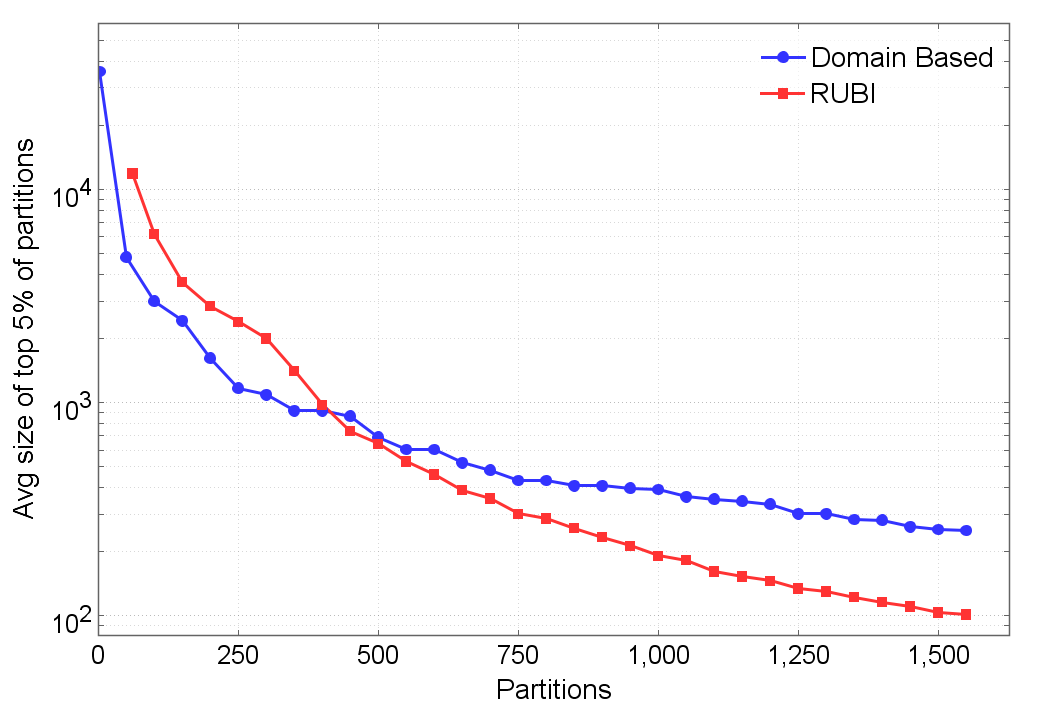
\includegraphics[width=1.0\columnwidth]{OldvsNewAvgSize}
%\caption{Initially, domain-based partitioning has a larger average size of partitions, leading to a higher initial performance. Note %that when all partitions are reward independent, domain-based partitioning had only a few number of very large partitions. RUBI %partitioning on the other hand included a much smaller average size, and many more partitions. }
%\label{OldvsNewAvgSize}
%\end{figure}

\begin{figure}
\centering
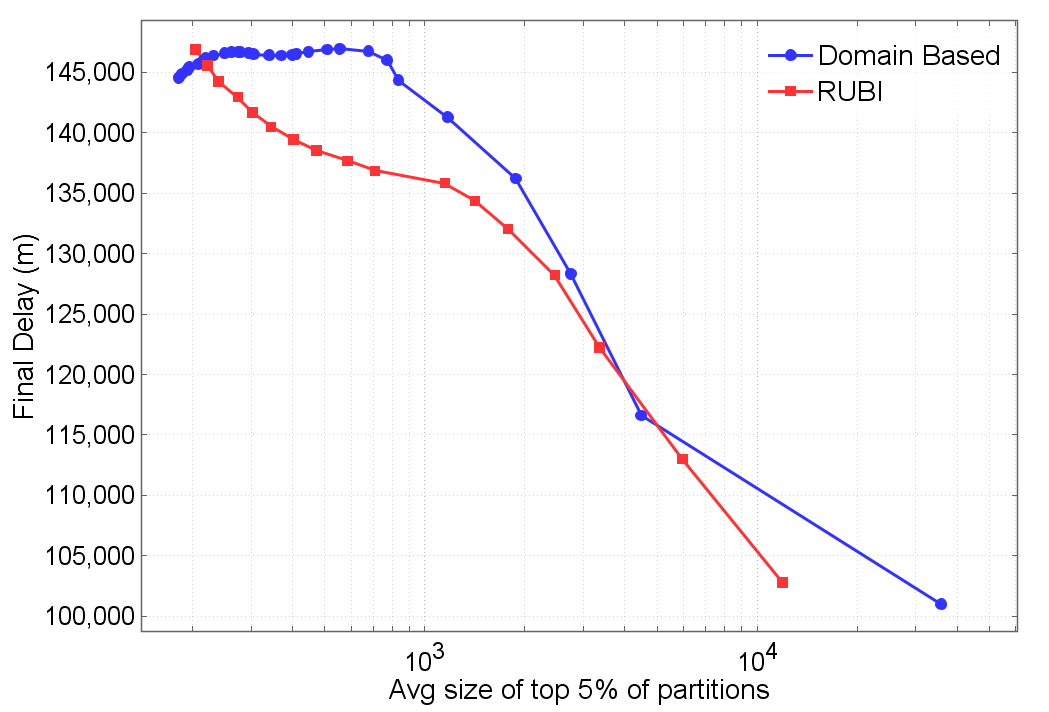
\includegraphics[width=1.0\columnwidth]{ATFMPPerformancevsAvgSize}
\caption{When comparing individual partition size averages to performance, RUBI partitions perform much better than domain specific partitions with respect to average partition size and final performance.}
\label{ATFMPPerformancevsAvgSize}
\end{figure}


\section{Conclusion}
This paper introduces RUBI, a partitioning algorithm that computes reward-based impacts that can then be used to partition agents together, removing the need for prior knowledge of the system. This method also removes the need develop similarity metrics derived from expert domain knowledge. Additionally, by removing all knowledge about the domain and partitioning based on reward, RUBI can be used to discover non-trivial indirect interactions encoded in a reward signal. Since RUBI uses only a reward signal to compute impacts, it will theoretically work in any domain where partitioning is useful.

In this work, we showed that partitioning with RUBI accurately encapsulated the amount of coupling between agents, leading to a higher self-similarity metric over the domain-based partitioning, leading to faster simulation computation times. Learning using partitions developed with RUBI also found a 37\% increase in performance over the greedy solution with a 510x reduction in time complexity per learning step  compared to the 450x speed up using domain-based partitioning. RUBI-based partitioning is able to achieve the same performance 10\% faster. This reduction in simulation cost was due to partitioning with RUBI leading to a larger number of smaller sized reward independent partitions.

Future work in RUBI would involve applying it to domains where coupling is very difficult to predict. We expect that RUBI would work fine in such a domain, but more exploration is needed. Performing a formal analysis of the relation between the number of iterations of RUBI and partition performance is important for future work, as we currently do not have a formal stop criteria. Approximating the impact score of each agent, rather than using a accumulation has the potential of being very informative when performing an analysis of a system. Future work in performing a simple approximation of the local reward function for each agent will greatly speed up RUBI computation time. Lastly, performing distributed clustering would be an important, yet simple extension to this work. Agents need only to compute the difference in local rewards if they come into contact with another agent, and then partition using this trimmed down similarity matrix. 
\label{sec:CONCLUSION}


\bibliographystyle{aaai}
\bibliography{thesis}

\end{document}
